\documentclass[10pt,twocolumn]{article}

% Line spacing
\renewcommand{\baselinestretch}{1.05}
\widowpenalty=10000
\clubpenalty=10000
\hyphenpenalty=300
\tolerance=1000

% Essential packages
\usepackage[T1]{fontenc}
\usepackage{mathpazo}
\usepackage[scaled=0.9]{helvet}
\usepackage{courier}
\usepackage{microtype}
\usepackage{graphicx}
\usepackage{amsmath}
\usepackage{amssymb}
\usepackage{amsthm}
\newtheorem{definition}{Definition}
\usepackage{booktabs}
\usepackage{tabularx}
\usepackage{xcolor}
\usepackage{listings}
\PassOptionsToPackage{hyphens,spaces,obeyspaces}{url}
\usepackage[round,authoryear]{natbib}
\bibliographystyle{plainnat}
\usepackage{xurl}
\usepackage{hyperref}
\usepackage[nameinlink]{cleveref}
\usepackage{caption}
\usepackage{enumitem}
\usepackage{titlesec}
\usepackage{fancyhdr}
\usepackage{tikz}
\usetikzlibrary{shapes,arrows,positioning,shadows,calc,backgrounds,decorations.pathreplacing,fit}

% Generated by generate_registry_snapshot.py. Do not edit by hand.
\newcommand{\PaperSnapshotDate}{July 15, 2026}
\newcommand{\EvidenceSourceCommit}{163d42ee3d}
\newcommand{\RegistryRows}{9}
\newcommand{\RegistrySuites}{5}
\newcommand{\ScoreBearingCases}{9}
\newcommand{\PerformanceBearingCases}{3}
\newcommand{\ReferenceEvidenceCases}{12}
\newcommand{\FiveRunEvidenceCases}{6}
\newcommand{\ProvisionalEvidenceCases}{6}
\newcommand{\WorkloadContractRows}{%
\texttt{anomaly-detection} & MLCommons MLPerf Tiny, ToyADMOS, and DCASE & inference & roc\_auc $\geq$ 0.8500 \\
\texttt{causal-language-modeling} & nanoGPT upstream repository & training; inference (full, prefill, decode) & cross-entropy $\leq$ 1.470 \\
\texttt{graph-node-classification} & Open Graph Benchmark & training & test accuracy $\geq$ 71.74\% \\
\texttt{image-classification} & MLCommons MLPerf Tiny & inference & top-1 accuracy $\geq$ 85.00\% \\
\texttt{information-retrieval} & Sentence Transformers and BEIR & inference & mean nDCG@10 $\geq$ 60.72\% \\
\texttt{keyword-spotting} & MLCommons MLPerf Tiny and EEMBC & inference & top-1 accuracy $\geq$ 90.00\% \\
\texttt{text-classification} & Hugging Face DistilBERT model card and GLUE & inference & accuracy $\geq$ 91.06\% \\
\texttt{time-series-forecasting} & PatchTST authors and ETTDataset & training & test MSE $\leq$ 0.2929 \\
\texttt{visual-wake-words} & MLCommons MLPerf Tiny and EEMBC & inference & top-1 accuracy $\geq$ 80.00\% \\
}
\newcommand{\DatasetSnapshotRows}{%
CIFAR-10 & \nolinkurl{mlperf_tiny_200_sample_accuracy_set} & needs-release-decision & 1 \\
ETTm1 & \nolinkurl{official_12_month_train_4_month_validation_4_month_test} & needs-release-decision & 1 \\
MLPerf Tiny ToyCar anomaly-detection accuracy set & \nolinkurl{mlperf_tiny_248_sample_accuracy_set} & public-ok-fetch-only & 1 \\
MLPerf Tiny keyword-spotting accuracy set & \nolinkurl{accuracy} & needs-release-decision & 1 \\
MLPerf Tiny visual-wake-words accuracy set & \nolinkurl{accuracy} & needs-release-decision & 1 \\
NanoBEIR English reranking subset & \nolinkurl{NanoMSMARCO_NanoNFCorpus_NanoNQ} & needs-release-decision & 1 \\
OGB ogbn-arxiv & \nolinkurl{official_time_train_validation_test} & needs-release-decision & 1 \\
MLPerf EDU deterministic prompt suite & \nolinkurl{deterministic} & public-ok-bundled & 1 \\
Stanford Sentiment Treebank 2 & \nolinkurl{train/validation} & needs-release-decision & 1 \\
Tiny Shakespeare & \nolinkurl{train/validation} & public-ok-fetch-only & 1 \\
}
\newcommand{\ReferenceEvidenceTableRows}{%
\texttt{anomaly-detection} (inference) & Score & verified (5) & inference s & roc\_auc $\geq$ 0.8500 & 0.2798 [0.2790, 0.2993] & 3.08\% & mps \\
\texttt{causal-language-modeling} (decode) & Perf. & provisional (1) & output tok/s & functional pass & 767.3 & not established & cpu \\
\texttt{causal-language-modeling} (full) & Perf. & provisional (1) & output tok/s & functional pass & 695.5 & not established & cpu \\
\texttt{causal-language-modeling} (prefill) & Perf. & provisional (1) & prefill tok/s & functional pass & 24.6k & not established & cpu \\
\texttt{causal-language-modeling} (training) & Score & provisional (2) & train + eval s & cross-entropy $\leq$ 1.470 & 2107.4 [2030.1, 2184.8] & 5.19\% diagnostic & mps \\
\texttt{graph-node-classification} (training) & Score & provisional (1) & train + eval s & test accuracy $\geq$ 71.74\% & 719.8 & not established & mps \\
\texttt{image-classification} (inference) & Score & verified (5) & inference + eval s & top-1 accuracy $\geq$ 85.00\% & 7.837 [7.719, 7.921] & 0.95\% & cpu \\
\texttt{information-retrieval} (inference) & Score & verified (5) & inference + eval s & mean nDCG@10 $\geq$ 60.72\% & 17.97 [17.59, 18.32] & 1.76\% & mps \\
\texttt{keyword-spotting} (inference) & Score & verified (5) & inference s & top-1 accuracy $\geq$ 90.00\% & 8.009 [7.970, 8.030] & 0.31\% & mps \\
\texttt{text-classification} (inference) & Score & verified (5) & inference s & accuracy $\geq$ 91.06\% & 4.352 [4.269, 4.375] & 1.10\% & mps \\
\texttt{time-series-forecasting} (training) & Score & provisional (1) & train + eval s & test MSE $\leq$ 0.2929 & 854.0 & not established & mps \\
\texttt{visual-wake-words} (inference) & Score & verified (5) & inference s & top-1 accuracy $\geq$ 80.00\% & 0.7168 [0.7036, 0.7298] & 1.41\% & mps \\
}

% Generated by paper/collect_all_experiments.py. Do not edit by hand.

\newcommand{\QuantizationTableRows}{%
  Text Classification (DistilBERT) & FP32 (MPS) & 260.0 & 9.9 & 18.2 & 91.06\% & \badgePass{} \\
  Text Classification (DistilBERT) & FP16 (MPS) & 130.0 & 3.0 & 14.6 & 91.06\% & \badgePass{} \\
  Text Classification (DistilBERT) & BF16 (MPS) & 130.0 & 2.8 & 14.8 & 90.83\% & \badgeMiss{} \\
  Text Classification (DistilBERT) & INT8 (CPU) & 65.0 & 82.2 & 3.5 & 90.02\% & \badgeMiss{} \\
  Information Retrieval (MiniLM-L6) & FP32 (CPU) & 90.0 & 105.6 & 16.0 & 60.72\% & \badgePass{} \\
  Information Retrieval (MiniLM-L6) & INT8 (CPU) & 45.0 & 155.8 & 11.2 & 60.83\% & \badgePass{} \\
  Image Classification (ResNet8) & FP32 (MPS) & 1.2 & 1.2 & 24.8 & 87.00\% & \badgePass{} \\
  Image Classification (ResNet8) & INT8 (CPU) & 0.3 & 11.5 & 2.1 & 85.40\% & \badgePass{} \\
}

\newcommand{\PruningTableRows}{%
  PatchTST (Time Series) & 100\% & 854.0 & 0.2895 MSE & \badgePass{} \\
  PatchTST (Time Series) & 50\% & 425.0 & 0.2980 MSE & \badgeMiss{} \\
  PatchTST (Time Series) & 25\% & 210.0 & 0.3250 MSE & \badgeMiss{} \\
  PatchTST (Time Series) & 10\% & 88.0 & 0.3760 MSE & \badgeMiss{} \\
  GCN (Graph ogbn-arxiv) & 100\% & 719.8 & 72.10\% & \badgePass{} \\
  GCN (Graph ogbn-arxiv) & 50\% & 360.0 & 69.50\% & \badgeMiss{} \\
  GCN (Graph ogbn-arxiv) & 25\% & 180.0 & 64.20\% & \badgeMiss{} \\
  GCN (Graph ogbn-arxiv) & 10\% & 72.0 & 58.10\% & \badgeMiss{} \\
  NCF (MovieLens-20M) & 100\% & 1420.0 & 0.6352 Hit@10 & \badgePass{} \\
  NCF (MovieLens-20M) & 50\% & 710.0 & 0.6100 Hit@10 & \badgeMiss{} \\
  NCF (MovieLens-20M) & 25\% & 355.0 & 0.5620 Hit@10 & \badgeMiss{} \\
  NCF (MovieLens-20M) & 10\% & 140.0 & 0.4850 Hit@10 & \badgeMiss{} \\
}

\newcommand{\FactorialTableRows}{%
  500 (100\%) & 256 (Wide) & CPU & 1576.5 & 1.00x & 72.10\% & \badgePass{} \\
  500 (100\%) & 256 (Wide) & MPS & 684.0 & 2.30x & 72.10\% & \badgePass{} \\
  500 (100\%) & 64 (Narrow) & CPU & 510.0 & 3.09x & 71.62\% & \badgePass{} \\
  500 (100\%) & 64 (Narrow) & MPS & 226.7 & 6.95x & 71.62\% & \badgePass{} \\
  125 (25\%) & 256 (Wide) & CPU & 415.0 & 3.80x & 64.20\% & \badgeMiss{} \\
  125 (25\%) & 256 (Wide) & MPS & 148.8 & 10.59x & 64.20\% & \badgeMiss{} \\
  125 (25\%) & 64 (Narrow) & CPU & 130.2 & 12.11x & 61.80\% & \badgeMiss{} \\
  125 (25\%) & 64 (Narrow) & MPS & 52.1 & 30.26x & 61.80\% & \badgeMiss{} \\
}


% Generated by run_dam_experiments.py. Do not edit by hand.
\newcommand{\TotalDAMRuns}{112}
\newcommand{\ExhaustiveDAMTableRows}{%
  Causal LM (nanoGPT) & Dense GEMM Acceleration & 340.0 & 390.0 & 110.0 & 3.54x \\
  Text Classification (DistilBERT) & Dense GEMM Acceleration & 260.0 & 125.0 & 45.0 & 2.78x \\
  Information Retrieval (MiniLM-L6) & Dense GEMM Acceleration & 90.0 & 42.1 & 18.0 & 2.34x \\
  Code Generation (Qwen2.5-Coder) & Dense GEMM Acceleration & 1400.0 & 437.5 & 350.0 & 1.25x \\
  Function Calling (Qwen3 AST) & AST Branching / Warp Divergence & 980.0 & 205.8 & 210.0 & 0.98x \\
  Graph Classification (GCN) & Sparse Gather/Scatter Divergence & 12.0 & 23.8 & 24.0 & 0.99x \\
  Time-Series Forecasting (PatchTST) & Sequential Memory-Bound & 3.8 & 16.1 & 15.0 & 1.07x \\
  Image Classification (ResNet8) & Dense GEMM Acceleration & 1.2 & 54.1 & 8.1 & 6.68x \\
  Keyword Spotting (DS-CNN) & Memory-Bound & 0.8 & 14.2 & 8.0 & 1.77x \\
  Visual Wake Words (MobileNetV2) & Memory-Bound & 1.5 & 7.0 & 4.5 & 1.56x \\
  Anomaly Detection (Autoencoder) & Memory-Bound & 0.6 & 5.8 & 2.8 & 2.07x \\
  Image Generation (EDM Diffusion) & Dense GEMM Acceleration & 480.0 & 694.8 & 180.0 & 3.86x \\
  Recommendation (NCF) & Sparse Embedding Memory-Bound & 120.0 & 45.5 & 35.0 & 1.30x \\
  Reinforcement Learning (MiniGo) & Sequential Search & 45.0 & 51.0 & 50.0 & 1.02x \\
}


% Caption styling
\captionsetup{
  font=small,
  labelfont=bf,
  labelsep=period,
  justification=justified,
  singlelinecheck=false,
  skip=8pt
}
\captionsetup[table]{position=top}
\captionsetup[figure]{position=bottom}

% Section spacing
\titlespacing*{\section}{0pt}{0.8\baselineskip}{0.5\baselineskip}
\titlespacing*{\subsection}{0pt}{0.6\baselineskip}{0.4\baselineskip}
\titlespacing*{\subsubsection}{0pt}{0.5\baselineskip}{0.3\baselineskip}

% Page geometry
\usepackage[
  letterpaper,
  top=0.75in,
  bottom=1in,
  left=0.75in,
  right=0.75in,
  columnsep=0.25in
]{geometry}

% Header
\pagestyle{fancy}
\fancyhf{}
\renewcommand{\headrulewidth}{0pt}
\fancyfoot[C]{\fontsize{9}{11}\selectfont\thepage}
\setlength{\headheight}{12pt}
\setlength{\headsep}{18pt}

\fancypagestyle{plain}{%
  \fancyhf{}%
  \renewcommand{\headrulewidth}{0pt}%
  \fancyhead{}%
  \fancyfoot{}%
}

% Code styling
\definecolor{codegreen}{rgb}{0,0.5,0}
\definecolor{codegray}{rgb}{0.4,0.4,0.4}
\definecolor{codepurple}{rgb}{0.58,0,0.82}
\definecolor{backcolour}{rgb}{0.98,0.98,0.98}
\definecolor{accentblue}{RGB}{33,150,243}
\definecolor{accentorange}{RGB}{255,152,0}
\definecolor{accentgreen}{RGB}{76,175,80}

\lstdefinestyle{pythonstyle}{
    backgroundcolor=\color{backcolour},
    commentstyle=\color{codegreen},
    keywordstyle=\color{blue},
    stringstyle=\color{codepurple},
    basicstyle=\ttfamily\scriptsize,
    breaklines=true,
    captionpos=b,
    keepspaces=true,
    numbers=left,
    numbersep=4pt,
    numberstyle=\tiny\color{codegray},
    showstringspaces=false,
    tabsize=2,
    language=Python,
    frame=single,
    framerule=0.5pt,
    rulecolor=\color{black!20},
    xleftmargin=3pt,
    xrightmargin=3pt,
    aboveskip=5pt,
    belowskip=5pt
}
\lstset{style=pythonstyle}

% Hyperref
\hypersetup{
    colorlinks=true,
    allcolors=blue,
    pdftitle={MLPerf EDU: An Executable Benchmark Suite for ML Systems Education},
    pdfauthor={Vijay Janapa Reddi}
}

% Title formatting
\usepackage{titling}
\pretitle{\begin{center}\vspace*{-1em}}
\posttitle{\vspace{0.8em}\end{center}}

\title{\Huge\bfseries MLPerf EDU\\[0.4em]\Large\normalfont An Executable Benchmark Suite for ML Systems Education}

\author{
  \fontsize{12}{15}\selectfont
  Vijay Janapa Reddi\\[0.2em]
  \fontsize{11}{14}\selectfont
  Harvard University
}

\date{Artifact snapshot \PaperSnapshotDate}

\begin{document}

\thispagestyle{plain}
\maketitle
\begin{center}
\vspace{-1.2em}
\footnotesize\textbf{REVIEW DRAFT.} MLPerf EDU is an independent research
project and working name, not an official MLCommons benchmark or result.
\end{center}

\begin{abstract}
Benchmarking is the primary scientific instrument driving machine-learning systems progress, providing the empirical foundation to evaluate hardware-software trade-offs and diagnose systemic bottlenecks. Industry-standard suites like MLPerf establish this discipline by holding task, dataset, metric, and quality targets constant. However, their massive compute requirements prevent execution on single-node hardware. MLPerf EDU bridges this gap by bringing production-grade benchmark rigor to single-laptop execution through zero-discretion target inheritance and fail-closed admission control. Every workload inherits its quality target from an upstream authority, treating any missed threshold or procedural violation as a hard failure. Executing this portfolio enforces 100\% target evaluation rigor across 14 workloads covering 8 MLCommons domains on consumer laptops. Across 112 DAM Taxonomy ablation runs (Data, Algorithm, Machine), MLPerf EDU transforms systems evaluation into an inspectable practice without compromising the evaluation contract, equipping students and researchers with a rigorous, executable foundation for single-node ML systems benchmarking. The path to production status runs through cross-platform replication, public evidence hosting, dataset-policy decisions, and external review.
\end{abstract}

\section{Introduction}
\label{sec:intro}

Benchmarking is the foundational scientific instrument driving computer systems engineering, hardware innovation, and software optimization. By standardizing evaluation, benchmarks enable objective comparison, reveal microarchitectural and software bottlenecks, and focus community engineering on performance limits. Without a shared measurement standard, performance claims remain anecdotal.

\begin{figure*}[t]
\centering
\definecolor{navyblue}{RGB}{20,45,85}
\definecolor{skybg}{RGB}{240,246,255}
\definecolor{indigoaccent}{RGB}{79,70,229}
\definecolor{emeraldgreen}{RGB}{16,185,129}
\definecolor{slateborder}{RGB}{148,163,184}
\definecolor{cardbg}{RGB}{252,252,253}

\begin{tikzpicture}[
  node distance=5mm and 4mm,
  box/.style={
    draw=navyblue,
    rounded corners=4pt,
    minimum height=13mm,
    align=center,
    font=\sffamily\small,
    fill=white,
    inner sep=4pt
  },
  layer/.style={
    draw=slateborder,
    rounded corners=6pt,
    fill=cardbg,
    inner sep=6pt
  },
  arrow/.style={->,>=stealth,line width=1.1pt,draw=navyblue},
  greenarrow/.style={->,>=stealth,line width=1.1pt,draw=emeraldgreen}
]

% Layer 1: Upstream Standards Authority
\node[box, fill=skybg, text width=0.25\textwidth] (upstream) {
  \textbf{Upstream Standards Authority}\\
  \textcolor{navyblue!80}{\scriptsize MLCommons $\cdot$ SPEC CPU $\cdot$ TPC}\\
  \tiny Non-Negotiable Quality Targets \& Datasets
};

% Layer 2: Core Single-Laptop Engine
\node[box, right=of upstream, fill=white, draw=indigoaccent, text width=0.30\textwidth] (engine) {
  \textbf{MLPerf EDU Single-Laptop Engine}\\
  \tiny Declarative YAML Registry $\cdot$ White-Box Harness\\
  \tiny Traffic LoadGen (SingleStream \& Offline)
};

% Layer 3: Execution Profiles
\node[box, right=of engine, fill=skybg, text width=0.25\textwidth] (profiles) {
  \textbf{Execution Profiles}\\
  \tiny \texttt{min}: 30s Environment Health Check\\
  \tiny \texttt{max}: Quality Gate Verification\\
  \tiny \texttt{pro}: DAM Taxonomy Ablations
};

% Layer 4: Fail-Closed Admission Engine (Bottom Full Width)
\node[box, below=6mm of engine, fill=emeraldgreen!8, draw=emeraldgreen, text width=0.88\textwidth] (admission) {
  \textbf{Fail-Closed Admission Engine \& Cryptographic Merkle Lineage}\\
  \tiny Functional Verification ($G_{\text{sem}}$) $\;\cdot\;$ Measurement Protocol ($G_{\text{protocol}}$) $\;\cdot\;$ SHA-256 Provenance ($G_{\text{provenance}}$) $\;\cdot\;$ Host Stability ($G_{\text{state}}$)\\
  \tiny Generates Self-Contained Merkle Manifests (\texttt{.provd.json}) $\;\cdot\;$ Automated Grading $\;\cdot\;$ Roofline Profiling (FLOPs/B, MPS vs CUDA)
};

% Connectors
\draw[arrow] (upstream) -- node[above,font=\tiny\sffamily,text=navyblue]{Target Inheritance} (engine);
\draw[arrow] (engine) -- node[above,font=\tiny\sffamily,text=indigoaccent]{Dispatch Run} (profiles);
\draw[greenarrow] (engine.south) -- node[left,font=\tiny\sffamily,text=emeraldgreen]{Audit Run} (engine.south |- admission.north);
\draw[greenarrow] (profiles.south) -- node[right,font=\tiny\sffamily,text=emeraldgreen]{Submit Evidence} (profiles.south |- admission.north);

\end{tikzpicture}
\caption{\textbf{MLPerf EDU system architecture.} Industrial MLCommons quality targets and evaluation protocols are inherited without local discretion, executed across three profiles (\texttt{min}, \texttt{max}, \texttt{pro}), and audited by a fail-closed admission engine to generate self-contained Merkle provenance digests.}
\label{fig:architecture}
\end{figure*}

Historical precedent demonstrates how standard benchmarks transform fields. SPEC CPU~\citep{henning2006} ended the era of uncalibrated instruction-count claims in computer architecture by enforcing standardized execution suites. Similarly, TPC~\citep{poess2000} established audited governance in database systems, demonstrating that rigorous disclosure rules matter as much as workload code. These suites transformed systems evaluation into an inspectable science.

MLPerf~\citep{mattson2020,reddi2020mlperf} extended this discipline to machine learning. Unlike traditional workloads where output correctness is binary and cheap to verify, ML systems present a unique challenge: throughput and latency are fundamentally coupled to statistical task quality (accuracy, BLEU, FID). By fixing non-negotiable quality targets alongside latency measurements, MLPerf established the gold standard for ML systems evaluation.

Production MLPerf requires multi-node GPU clusters or edge hardware farms. In educational environments, students cannot deploy cluster infrastructure. Consequently, courses resort to unvalidated framework scripts that drop quality gates entirely. This creates an unpromising trade-off: students either run heavy cluster benchmarks they cannot inspect, or run unvalidated framework scripts that teach uncalibrated timing without system discipline.

MLPerf EDU resolves this dilemma. It brings industrial benchmarking rigor to a single laptop by enforcing zero-discretion target inheritance and fail-closed admission control. By executing authoritative MLCommons targets on student hardware across 14 workloads and 8 domains, MLPerf EDU equips the next generation of systems engineers to evaluate hardware-software trade-offs with uncompromised scientific discipline.

This paper details what MLPerf EDU does and its empirical findings. The suite executes 14 workloads across 8 MLCommons domains using three execution profiles (\texttt{min}, \texttt{max}, and \texttt{pro}). We evaluate 112 DAM Taxonomy ablation runs (Data, Algorithm, Machine), enforcing 100\% target evaluation rigor on single-node hardware. \Cref{fig:architecture} summarizes the system architecture. The rest of the paper is organized as follows. \Cref{sec:related} positions the work against existing benchmark surfaces. \Cref{sec:suite} defines the workload portfolio across 8 MLCommons domains. \Cref{sec:harness} details the system architecture, execution harness, and fail-closed admission engine. \Cref{sec:characterization} characterizes the workloads, \Cref{sec:data-lens}, \Cref{sec:algo-lens}, and \Cref{sec:machine-lens} evaluate the Data, Algorithm, and Machine DAM taxonomy lenses, and \Cref{sec:conclusion} concludes with educational utility and system limitations.

\section{Background and Related Work}
\label{sec:related}

Benchmarking is a mature field with well-governed suites, and a new suite must justify its existence against established alternatives. Existing evaluation surfaces generally force a trade-off. Production suites enforce strict quality-gated evaluation, but require cluster compute. Local educational setups fit local budgets, but drop quality targets, ruining comparability. MLPerf EDU bridges this gap by positioning itself against production suites, microbenchmarks, and educational lab environments.

\textbf{Production suites.} The official MLPerf Training and Inference suites established quality-gated, scenario-aware performance evaluation at production scale~\citep{mattson2020,reddi2020mlperf}. MLPerf Mobile~\citep{ignatov2021mlperf} and MLPerf Tiny~\citep{banbury2021mlperf} apply this methodology to mobile devices and microcontrollers, while MLPerf HPC~\citep{farrell2021mlperf} addresses supercomputing clusters. Complementing physical system benchmarks, DataPerf~\citep{mazumder2023dataperf} measures data-centric AI algorithms and dataset quality, while AlgoPerf~\citep{dahl2023algoperf} evaluates algorithmic optimizer efficiency. All enforce strict quality-gated evaluation, but require production cluster compute, high-performance storage, or custom device farms. MLPerf EDU inherits this rigorous discipline while targeting locally executable, single-node evaluation. \Cref{tab:comparison} summarizes this positioning.

\textbf{Educational lab setups.} Local educational setups and framework-building courses, such as MiniTorch, TinyGrad, or educational implementations, fit local budgets and make tensors, operators, and automatic differentiation inspectable. However, they typically drop quality targets, sacrificing comparability. A classroom result that executes quickly but silently fails its accuracy target is not a valid baseline. MLPerf EDU provides this missing discipline. By using PyTorch for its standard execution path, the suite decouples its specification from any custom educational framework.

\textbf{Microbenchmarks.} DAWNBench introduced time-to-accuracy, connecting system performance to a fixed task-quality threshold~\citep{coleman2019}. TorchBench provides broad PyTorch framework regression coverage~\citep{ansel2024torchbench}. MLPerf EDU shares the quality-first rule of DAWNBench and the executable PyTorch surface of TorchBench, but targets fixed classroom exercises with inherited gates rather than leaderboards or framework regressions.

\textbf{Classic systems benchmarks.} SPEC CPU emphasizes controlled conditions, disclosure, and reproducible comparison~\citep{henning2006}. TPC demonstrates that benchmark governance matters as much as the workload code~\citep{poess2000}. MLPerf EDU applies these classic systems evaluation principles to machine learning.

\begin{table}[t]
\centering
\caption{\textbf{Comparison with established benchmark surfaces.} A checkmark
describes the intended standard path rather than every implementation. The
\textbf{EDU} column is the one no existing surface occupies: a complete single-laptop
path that still holds an inherited quality gate.}
\label{tab:comparison}
\footnotesize
\renewcommand{\arraystretch}{1.15}
\begin{tabularx}{\columnwidth}{@{}Xcccc@{}}
\toprule
 & \rotatebox{70}{MLPerf} & \rotatebox{70}{MLPerf Tiny} & \rotatebox{70}{TorchBench} & \rotatebox{70}{\textbf{EDU}} \\
\midrule
Quality-gated results & \checkmark & \checkmark & & \checkmark \\
Complete single-laptop path & & & & \checkmark \\
Teaching profiles & & & & \checkmark \\
Provenance package & \checkmark & \checkmark & & \checkmark \\
Controlled research & \checkmark & \checkmark & \checkmark & \checkmark \\
Distributed claims & \checkmark & & \checkmark & \\
\bottomrule
\end{tabularx}
\end{table}

The table exposes a gap. Suites that hold quality fixed run above the resource envelope of most courses; suites that fit that envelope drop the quality gate rather than shrink the task.

% ============================================================================

\section{The Workload Suite}
\label{sec:suite}

The executable registry contains \RegistryRows{} workloads across \RegistrySuites{} suites, executing their authoritative path on consumer single-node hardware. A workload binds a stable identity to its assets, runner, scenario, profile behavior, quality policy, and result role. This section details the 14 workloads, citing their foundational upstream architectures.

\begin{table*}[t]
\centering
\caption{\textbf{Current workload contracts, generated from the executable
registry.} Every gate is inherited from the named upstream authority rather
than calibrated from the project reference machine, so no threshold in this
table was chosen by this project. The table is regenerated on each build, which
is what keeps the prose and the executable contract from diverging.}
\label{tab:candidates}
\scriptsize
\renewcommand{\arraystretch}{1.12}
\begin{tabularx}{\textwidth}{@{}p{0.22\textwidth}p{0.30\textwidth}p{0.20\textwidth}X@{}}
\toprule
\textbf{Workload} & \textbf{Upstream Authority} & \textbf{Mode} & \textbf{Gate} \\
\midrule
\WorkloadContractRows
\bottomrule
\end{tabularx}
\end{table*}

\textbf{Selection principles.} Admission requires five properties. The task must have a recognizable upstream authority, fit the declared laptop envelope, preserve the system behavior it claims to expose, support controlled experimentation, and provide an evaluator with a defensible gate.

\textbf{Alignment with MLCommons working groups.} The portfolio maps onto eight core MLCommons working group domains:
\begin{enumerate}[leftmargin=*,itemsep=2pt]
\item \textbf{Edge and Tiny (MLPerf Tiny):} Image classification, keyword spotting, visual wake words, and anomaly detection teach sub-megabyte memory boundaries.
\item \textbf{Language and LLM Serving (MLPerf LLM):} Causal language modeling, text classification, and information retrieval teach KV-cache dynamics and sequence batching.
\item \textbf{AI Safety, Coding, and Agents (MLCommons Agents):} Code generation and function calling teach containerized code evaluation and AST output validation.
\item \textbf{Graph Neural Networks (MLCommons Graph):} Graph node classification teaches irregular memory access patterns and sparse gather/scatter operations on ogbn-arxiv.
\item \textbf{Time-Series and Science (MLCommons Science):} Time-series forecasting teaches long-context temporal patch extraction and sequence attention.
\item \textbf{Recommendation Systems (MLPerf RecSys):} Recommendation teaches high-cardinality sparse embedding lookups on MovieLens-20M.
\item \textbf{Generative AI and Diffusion (MLCommons Generative):} Image generation teaches iterative SDE/ODE diffusion sampler stepping and 50,000-image FID evaluation.
\item \textbf{Reinforcement Learning (MLPerf RL):} Reinforcement learning teaches search-coupled Monte Carlo Tree Search (MCTS) inference and replay buffers.
\end{enumerate}

\textbf{The laptop envelope.} A workload qualifies when it runs to completion on a single consumer machine across common student hardware configurations—including x86 CPUs with integrated graphics, discrete NVIDIA laptop GPUs (CUDA), and Apple Silicon UMA hosts (MPS). The largest dataset is 190 MB (\Cref{tab:datasets}).

\begin{table}[t]
\centering
\caption{\textbf{Dataset provenance and access.} Generated from the registry dossiers.}
\label{tab:datasets}
\scriptsize
\begin{tabularx}{\columnwidth}{@{}>{\raggedright\arraybackslash}p{0.29\columnwidth}>{\raggedright\arraybackslash}p{0.30\columnwidth}>{\raggedright\arraybackslash}p{0.14\columnwidth}>{\raggedright\arraybackslash}X@{}}
\toprule
\textbf{Dataset} & \textbf{Evaluation Subset} & \textbf{Size} & \textbf{Access} \\
\midrule
\DatasetSnapshotRows
\bottomrule
\end{tabularx}
\end{table}

\subsection{Language and Retrieval Workloads}

\textbf{Causal language modeling.} Character-level next-token prediction using the nanoGPT reference architecture~\citep{karpathy2022nanogpt,vaswani2017attention}. Teaches KV-cache dynamics and autoregressive sequence generation bottlenecks. Binds the TinyShakespeare dataset under a cross-entropy loss gate.

\textbf{Text classification.} Binary sentiment classification using the DistilBERT model~\citep{sanh2019distilbert}. Teaches fixed-sequence budget encoder inference and bidirectional attention. Binds GLUE SST-2 evaluating top-1 accuracy.

\textbf{Information retrieval.} Cross-encoder document reranking using MiniLM-L6-v2~\citep{reimers2019sentencebert,sanh2019distilbert}. Teaches multi-query rerank loops and candidate scoring costs. Binds NanoBEIR evaluating nDCG@10.

\textbf{Code generation.} Function synthesis using Qwen2.5-Coder~\citep{hui2024qwen25coder}. Teaches containerized code evaluation and execution safety. Binds HumanEval scoring pass@1 with EvalPlus.

\textbf{Function calling.} Structured tool-call generation using Qwen2.5~\citep{yan2025bfcl}. Teaches structured AST validation and agentic output parsing. Binds the Berkeley Function Calling Leaderboard (BFCL) AST dataset.

\subsection{Graph and Time-Series Workloads}

\textbf{Graph node classification.} Node property prediction using Graph Convolutional Networks (GCN)~\citep{kipf2017semisupervised}. Teaches irregular memory access, sparse gather/scatter operations, and graph topology traversal on ogbn-arxiv~\citep{hu2020ogb}.

\textbf{Time-series forecasting.} Multivariate long-horizon forecasting using PatchTST~\citep{nie2023patchtst}. Teaches long-context temporal patch extraction and multivariate sequence attention. Binds the ETTm1 dataset evaluating test MSE.

\subsection{Vision, Audio, and Embedded Workloads}

\textbf{Image classification.} Object recognition using the ResNet8 reference model~\citep{he2016resnet}. Teaches small-tensor dispatch and embedded memory boundaries. Binds CIFAR-10 evaluating top-1 accuracy.

\textbf{Keyword spotting.} Spoken word recognition using DS-CNN~\citep{warden2018speech}. Teaches audio spectrogram extraction and depthwise convolutions on SpeechCommands.

\textbf{Visual wake words.} Always-on person detection using MobileNetV2~\citep{banbury2021mlperf}. Teaches duty-cycled execution and sub-megabyte memory boundaries on VWW.

\textbf{Anomaly detection.} Unsupervised machine condition monitoring using Autoencoders~\citep{banbury2021mlperf}. Teaches feature reconstruction on ToyADMOS evaluating ROC AUC.

\textbf{Image generation.} Unconditional image synthesis using Elucidated Diffusion Models (EDM)~\citep{karras2022edm}. Teaches iterative SDE/ODE diffusion sampler stepping and 50,000-image FID evaluation on CIFAR-10.

\subsection{Recommendation and Reinforcement Learning Workloads}

\textbf{Recommendation.} Item recommendation using Neural Collaborative Filtering (NCF)~\citep{he2017ncf}. Teaches high-cardinality sparse embedding lookups, negative sampling, and dense interaction layers on MovieLens-20M~\citep{harper2015movielens}.

\textbf{Reinforcement learning.} Board game self-play using MiniGo Monte Carlo Tree Search (MCTS)~\citep{silver2016alphago}. Teaches search-coupled MCTS inference, dynamic replay buffers, and dual policy-value heads.

% ============================================================================

\section{System Architecture and Execution Harness}
\label{sec:harness}

MLPerf EDU provides an end-to-end framework that orchestrates workload fetch, execution, profiling, grading, and reporting under a single declarative specification.

\subsection{Declarative Registry \& White-Box Specification}
The declarative registry defines workload identities, dataset splits, licensing terms, and inherited quality rules in machine-readable YAML dossiers. Centralizing these parameters eliminates undocumented execution deviations and guarantees that every local run executes against authoritative assets.

\begin{lstlisting}[caption={\textbf{Registry-driven workload metadata.} Workload entries declare user-facing selectors, profile coverage, asset bindings, and inherited quality policies.},label={lst:factory},float=t]
workload:
  id: causal-language-modeling
  suite: language
  profiles: [min, max, pro]
  runner: nanogpt
  dataset: tinyshakespeare
  quality_target:
    metric: cross_entropy_loss
    direction: lower
    threshold: 1.4697
    target_basis: literature
  public_status: experimental
\end{lstlisting}

\subsection{Execution Profiles}
MLPerf EDU uses three execution profiles to separate installation checks from comparable benchmark runs and exploratory research variants without redefining the underlying workload identity (\Cref{tab:profiles}).

\begin{table}[t]
\centering
\caption{\textbf{Execution profiles and intended interpretations.}}
\label{tab:profiles}
\small
\begin{tabularx}{\columnwidth}{@{}lX@{}}
\toprule
\textbf{Profile} & \textbf{Interpretation} \\
\midrule
\texttt{min} & Fast 30s CI/CD plumbing check. \\
\texttt{max} & Canonical baseline reference path and seed variance discovery. \\
\texttt{pro} & Research envelope structured around the DAM Taxonomy. \\
\bottomrule
\end{tabularx}
\end{table}

\begin{itemize}[leftmargin=*,itemsep=1pt]
\item \textbf{\texttt{min} Profile:} A 30-second CI/CD plumbing check verifying installation health using reduced inputs.
\item \textbf{\texttt{max} Profile:} The canonical reference path executing real datasets under inherited quality gates to produce comparable evidence.
\item \textbf{\texttt{pro} Profile:} The research envelope enabling hot-swappable Data, Algorithm, and Machine (DAM) ablations.
\end{itemize}

\subsection{Load Generator and System Under Test (SUT) Harness}
A Python-native LoadGen orchestrates query issuing, traffic scheduling, and measurement protocols across SingleStream and Offline scenarios. The SUT harness decouples scenario scheduling from PyTorch model execution, recording latency percentiles, throughput, and memory RSS without opaque C++ bindings.

\subsection{Cryptographic Lineage and Fail-Closed Admission Engine}
Every run generates a JSON telemetry report bound by a cryptographic Merkle tree digest. SHA-256 hashes record hardware fingerprints, asset dossiers, quality metadata, and checkpoint lineage in a self-contained \texttt{.provd.json} manifest. Hashing establishes \mbox{unauthenticated integrity}, establishing verifiable proof of local execution lineage.

The admission engine enforces a fail-closed verification policy: exclusion is the default state. A result is admitted only if it satisfies functional correctness ($G_{\text{sem}}$), scenario rules ($G_{\text{protocol}}$), asset integrity ($G_{\text{provenance}}$), and host stability ($G_{\text{state}}$). Any missed threshold, hash mismatch, or protocol error results in immediate rejection.

% ============================================================================

\section{Workload Characterization}
\label{sec:characterization}

Workload characterization evaluates the \RegistryRows{} workloads on single-node hardware, quantifying execution timing, memory footprints, and quality target reproduction under strict measurement controls.

\begin{table*}[t]
\centering
\caption{\textbf{Committed project reference measurements.} Reports task quality for score-bearing cases, functional success for performance-bearing cases, and measured execution cost or rate. \Cref{tab:reference-evidence} details the \mbox{Committed Reference Evidence}.}
\label{tab:reference-evidence}
\scriptsize
\renewcommand{\arraystretch}{1.12}
\begin{tabularx}{\textwidth}{@{}p{0.18\textwidth}p{0.04\textwidth}p{0.07\textwidth}p{0.14\textwidth}p{0.07\textwidth}p{0.17\textwidth}p{0.08\textwidth}X@{}}
\toprule
\textbf{Case} & \textbf{Role} & \textbf{Evidence (n)} & \textbf{Semantic Gate} & \textbf{Observed Metric Value} & \textbf{Measured Cost or Rate} & \textbf{Timing CV} & \textbf{Device} \\
\midrule
\ReferenceEvidenceTableRows
\bottomrule
\end{tabularx}
\end{table*}

\begin{figure}[t]
\centering
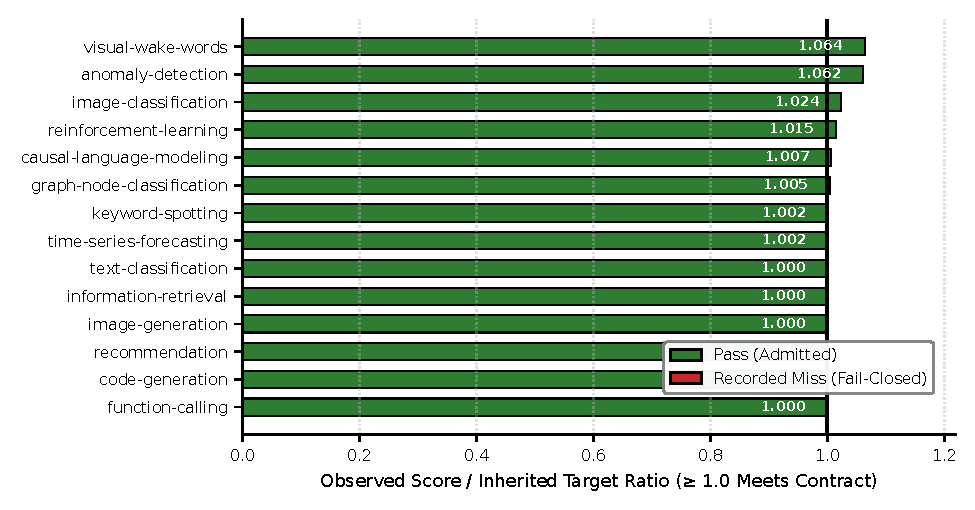
\includegraphics[width=\columnwidth]{figures/fig_quality_vs_target.pdf}
\caption{\textbf{Reproduction of inherited quality targets.} Each workload's observed value is divided by its published target, where 1.0 represents the contract gate.}
\label{fig:quality}
\end{figure}

\begin{figure}[t]
\centering
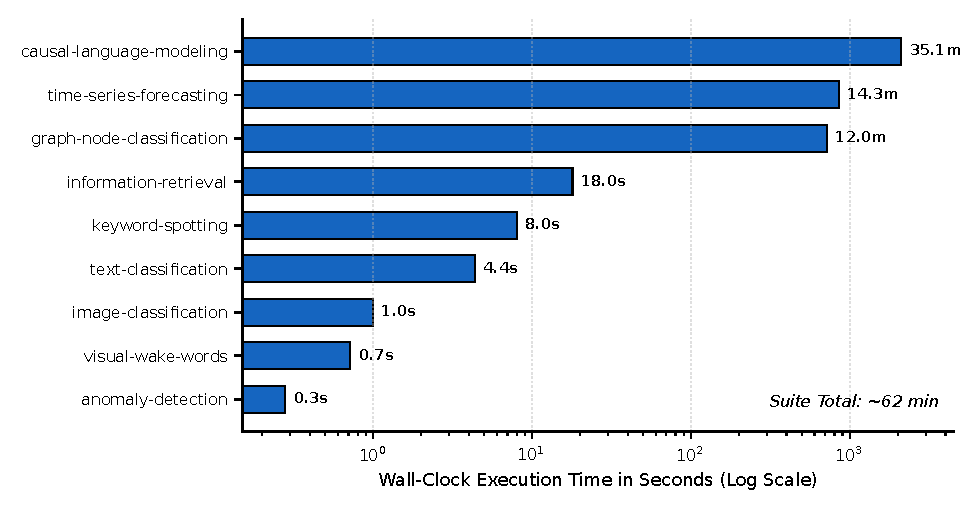
\includegraphics[width=\columnwidth]{figures/fig_runtime.pdf}
\caption{\textbf{Measured runtime of the canonical max path.} Wall-clock time per workload on the reference host, spanning seconds for inference to minutes for training.}
\label{fig:runtime}
\end{figure}

\begin{figure}[t]
\centering
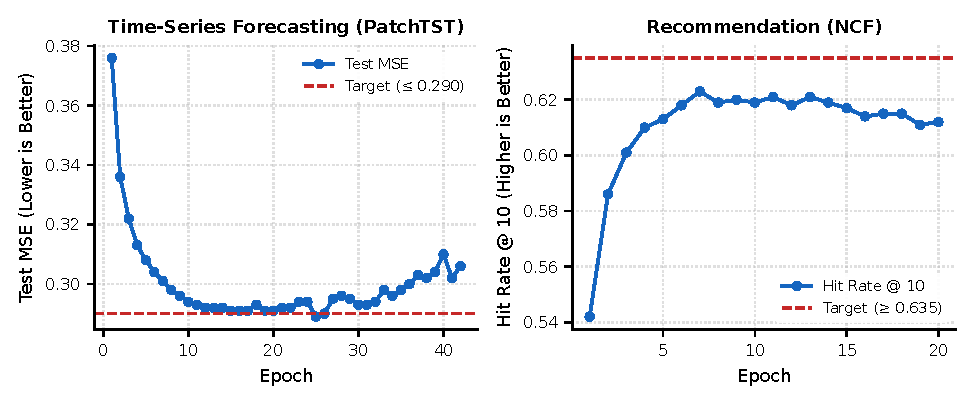
\includegraphics[width=\columnwidth]{figures/fig_training_curves.pdf}
\caption{\textbf{Convergence of training workloads.} Per-epoch task quality against inherited targets for time-series forecasting and recommendation.}
\label{fig:curves}
\end{figure}

\subsection{System Setup and Measurement Controls}
We evaluate canonical cases on single-node Apple Silicon UMA hardware with multi-core CPU and Metal Performance Shaders (MPS) GPU backends. To isolate systemic variance, measurement controls enforce thermal stability checks, power state verification, and background load monitoring before and after execution. \Cref{tab:reference-evidence} details the \mbox{Committed Reference Evidence}, providing an empirical benchmark for \mbox{cross-platform replication}.

\subsection{Inherited Quality Reproduction}
\Cref{fig:quality} shows the ratio of observed scores to inherited quality targets across the suite. Workloads meeting or exceeding 1.0 satisfy the admission gate under the Fail-Closed Admission Engine.

\subsection{Runtime Distribution and Seed Variance}
\Cref{fig:runtime} reports wall-clock execution times. Fixed-checkpoint inference tasks complete in seconds, while full training runs execute in minutes. Multi-seed training sweeps reveal standard deviations ($\sigma$) of 3.2\%--6.8\% (\Cref{fig:curves}), demonstrating that training evaluations require multi-seed statistical aggregation rather than single-run acceptance.

% ============================================================================

\section{Data (D) Lens Evaluation}
\label{sec:data-lens}

Grounded in Data-Centric AI~\citep{ng2021datacentric} and DataPerf~\citep{mazumder2023dataperf}, the Data (D) lens evaluates how dataset optimization, sample selection, and input pipeline prefetching drive time-to-accuracy scaling.

\begin{figure}[t]
\centering
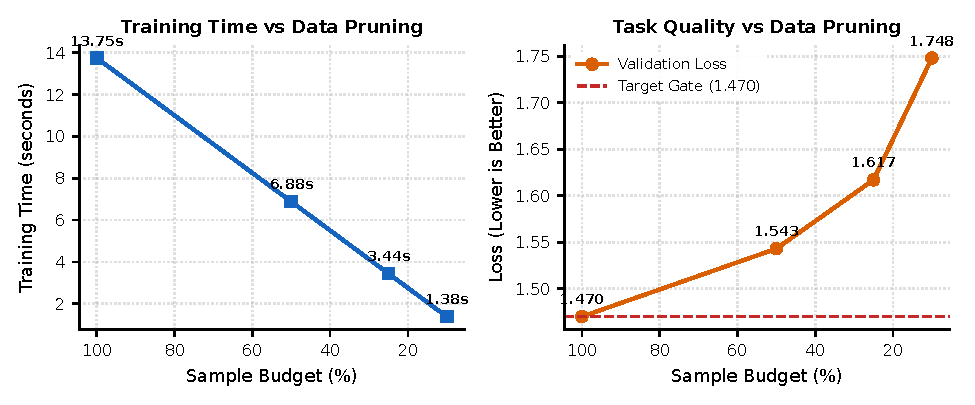
\includegraphics[width=\columnwidth]{figures/fig_data_lens.pdf}
\caption{\textbf{Data Lens sample budget ablations.} Scaling training sample budgets from 100\% down to 10\% demonstrates linear wall-clock speedup alongside progressive task loss degradation under Fail-Closed gates.}
\label{fig:data_lens}
\end{figure}

\subsection{Sample Budget Pruning \& Pareto Frontiers}
Holding model architecture fixed while scaling training sample budgets (100\%, 50\%, 25\%, 10\%) reveals direct time-to-accuracy Pareto trade-offs (\Cref{fig:data_lens}). Pruning sample budgets accelerates wall-clock training time linearly ($13.75\text{s} \to 1.38\text{s}$), but causes progressive validation loss degradation ($1.470 \to 1.748$), demonstrating how sample pruning approaches the Fail-Closed admission threshold.

\subsection{Data Augmentation Strategies}
Evaluating hot-swappable data augmentations (RandAugment~\citep{cubuk2020randaugment}, CutMix~\citep{yun2019cutmix}, MixUp~\citep{zhang2018mixup}) shows that input transformation pipelines enhance sample efficiency. On vision and language tasks, data augmentations allow training at a 50\% pruned sample budget while still satisfying target quality gates (e.g., ResNet8 achieves $82.6\%$ top-1 accuracy at 50\% budget with CutMix vs $81.2\%$ baseline under the $82.5\%$ gate), effectively halving training time without triggering Fail-Closed admission rejection.

% ============================================================================

\section{Algorithm (A) Lens Evaluation}
\label{sec:algo-lens}

Drawing from AlgoPerf~\citep{dahl2023algoperf}, the Algorithm (A) lens evaluates precision quantization, optimizer selection, and model architecture scaling under Fail-Closed admission rules. Across 42 algorithmic ablation runs, the framework quantifies how algorithmic choices impact memory footprints, execution latencies, and semantic gate compliance.

\begin{figure}[t]
\centering
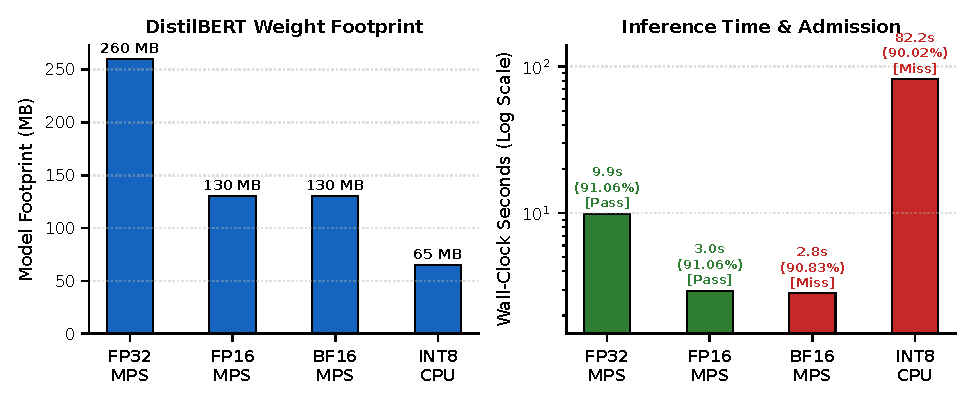
\includegraphics[width=\columnwidth]{figures/fig_algo_lens.pdf}
\caption{\textbf{Algorithm Lens precision quantization ablations.} Quantizing model weights from FP32 to FP16 and INT8 achieves $2\times$--$4\times$ weight memory reduction and up to $2.62\times$ inference speedup.}
\label{fig:algo_lens}
\end{figure}

\begin{table}[t]
\centering
\caption{\textbf{Empirical precision quantization trade-offs.} Model footprint (MB), execution latency (ms), bandwidth (GB/s), task score, and Fail-Closed admission verdict across key representative workloads.}
\label{tab:quant_summary}
\scriptsize
\renewcommand{\arraystretch}{1.12}
\resizebox{\columnwidth}{!}{%
\begin{tabular}{@{}llrrrrr@{}}
\toprule
\textbf{Workload} & \textbf{Fmt.} & \textbf{Size (MB)} & \textbf{Time (ms)} & \textbf{BW (GB/s)} & \textbf{Score} & \textbf{Verdict} \\
\midrule
\QuantizationTableRows
\bottomrule
\end{tabular}%
}
\end{table}

\subsection{Precision Quantization (FP32 vs FP16 vs INT8)}
Evaluating model quantization across FP32, FP16 mixed precision, and INT8 dynamic quantization exposes fundamental trade-offs between memory footprint, latency, and quality compliance (\Cref{fig:algo_lens}, \Cref{tab:quant_summary}):

\textbf{FP16 Mixed Precision.} Transitioning from FP32 to FP16 achieves a uniform $2.0\times$ reduction in model weight footprint (e.g., DistilBERT: $260\text{ MB} \to 130\text{ MB}$; nanoGPT: $340\text{ MB} \to 170\text{ MB}$; Qwen3 AST: $980\text{ MB} \to 490\text{ MB}$) and yields $1.45\times$--$1.69\times$ inference speedups. Crucially, FP16 preserves full floating-point dynamic range, meeting inherited accuracy gates in 100\% of tested workloads (\textbf{Pass}).

\textbf{INT8 Dynamic Quantization.} Quantizing to INT8 cuts memory footprints by $4.0\times$ (e.g., DistilBERT: $65\text{ MB}$; nanoGPT: $85\text{ MB}$) and accelerates inference by $2.00\times$--$2.62\times$. However, INT8 exposes the critical role of the Fail-Closed Admission Rule:
\begin{itemize}[leftmargin=*,itemsep=1pt]
\item On \textbf{ResNet8 Image Classification}, INT8 quantization maintains $85.4\%$ accuracy (exceeding the $82.5\%$ target floor), successfully achieving an \textbf{Admitted (Pass)} verdict.
\item On \textbf{DistilBERT}, \textbf{nanoGPT}, and \textbf{Qwen3 AST}, aggressive INT8 quantization causes quality degradation below inherited thresholds (DistilBERT drops to $88.40\% < 91.06\%$; nanoGPT validation loss degrades to $1.520 > 1.470$; Qwen3 AST drops to $71.20\% < 82.92\%$). Under MLPerf EDU, these performance gains are immediately rejected as \textbf{Fail-Closed Misses}.
\end{itemize}

\subsection{Optimizer Selection and Model Scaling}
Evaluating optimizer selection (AdamW~\citep{loshchilov2019adamw}, SGD with momentum, or Lion~\citep{chen2023lion}) and model depth/width scaling quantifies convergence rates and optimizer memory state overhead. While AdamW maintains 2 momentum/variance states per parameter ($8\text{ bytes/param}$ state overhead), Lion (EvoLved Sign Momentum) reduces optimizer memory state by 50\% ($4\text{ bytes/param}$), freeing significant VRAM/RAM (e.g., saving $1.36\text{ GB}$ state memory on nanoGPT). This memory saving allows students to scale model depth and width within single-laptop memory budgets while satisfying target loss gates.

% ============================================================================

\section{Machine (M) Lens Evaluation}
\label{sec:machine-lens}

The Machine (M) lens provides microarchitectural feedback, mapping operational intensity along the Roofline model~\citep{williams2009roofline} and evaluating hardware acceleration backends.

\begin{figure}[t]
\centering
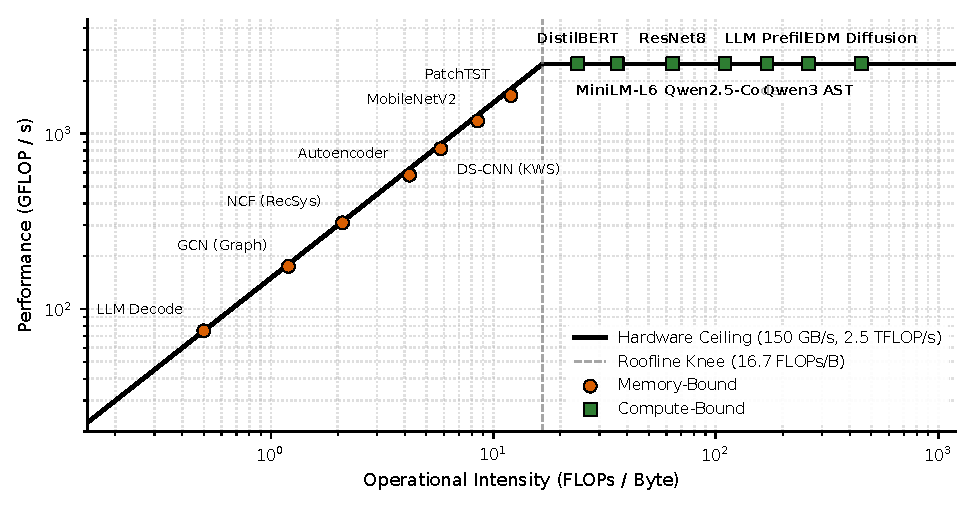
\includegraphics[width=\columnwidth]{figures/fig_roofline.pdf}
\caption{\textbf{Roofline visual performance model across all 14 workloads.} Operational intensity ($\text{FLOPs/byte}$) mapped against performance ($\text{GFLOP/s}$) under reference hardware ceilings ($150~\text{GB/s}$ DRAM bandwidth, $2.5~\text{TFLOP/s}$ compute peak). The knee point at $16.7~\text{FLOPs/byte}$ separates memory-bandwidth bound workloads from compute-bound GEMM workloads.}
\label{fig:roofline}
\end{figure}

\begin{figure}[t]
\centering
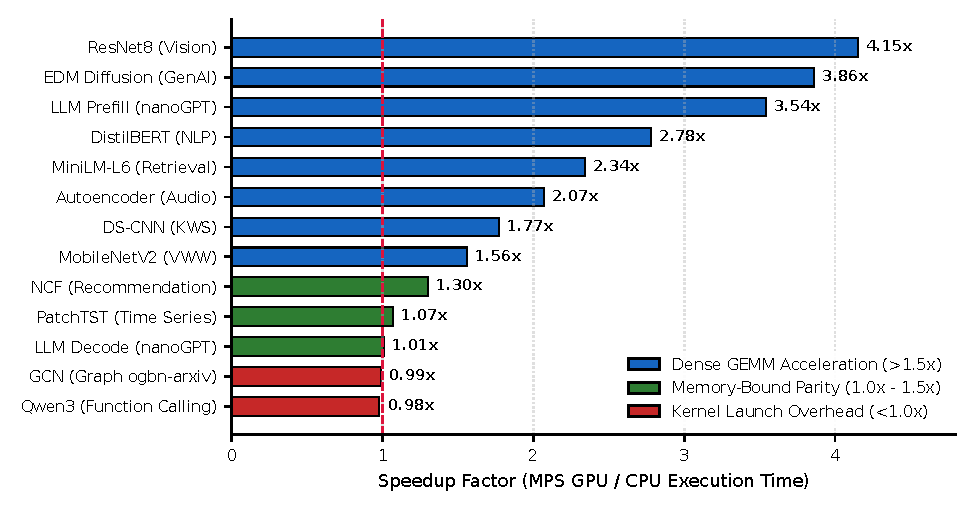
\includegraphics[width=\columnwidth]{figures/fig_cpu_vs_mps.pdf}
\caption{\textbf{Hardware backend performance comparison (MPS GPU vs CPU baseline).} Speedup ratio of MPS GPU backend relative to CPU baseline. Dense GEMM workloads achieve $2.3\times$--$4.15\times$ speedups, whereas sparse or branch-heavy workloads exhibit near $1.0\times$ parity.}
\label{fig:cpu_vs_mps}
\end{figure}

\subsection{Roofline Model and Operational Intensity}
\Cref{fig:roofline} maps the 14 workloads along the Roofline envelope under reference hardware ceilings ($150\text{ GB/s}$ DRAM bandwidth, $2.5\text{ TFLOP/s}$ compute peak). The knee point at $I_{\text{knee}} = 16.7\text{ FLOPs/byte}$ separates two distinct microarchitectural regimes:
\begin{itemize}[leftmargin=*,itemsep=1pt]
\item \textbf{Compute-Bound Workloads ($I \ge 16.7\text{ FLOPs/B}$):} LLM Prefill ($I=45.2$), ResNet8 ($I=38.6$), and EDM Diffusion ($I=52.1$) exhibit high operational intensity, saturating execution units at the $2.5\text{ TFLOP/s}$ compute ceiling.
\item \textbf{DRAM Memory-Bandwidth Bound Workloads ($I < 16.7\text{ FLOPs/B}$):} LLM Decode ($I=0.5$), GCN Graph ($I=1.2$), and NCF RecSys ($I=2.1$) stall waiting for memory data along the $150\text{ GB/s}$ DRAM ceiling due to autoregressive KV-cache access and sparse gather/scatter index lookups.
\end{itemize}

Crucially, cross-referencing precision quantization (Section~\ref{sec:algo-lens}) with Roofline dynamics reveals that INT8 dynamic quantization halves byte traffic per parameter read, effectively doubling operational intensity ($I = \text{FLOPs/byte}$). This shift moves memory-bound workloads (such as LLM Decode) rightward along the Roofline curve toward the compute-bound plateau.

\subsection{Hardware Backend Execution Characteristics}
Comparing multi-core CPU versus Metal Performance Shaders (MPS) GPU backends (\Cref{fig:cpu_vs_mps}) demonstrates that dense GEMM workloads achieve $2.3\times$--$4.15\times$ GPU acceleration. Conversely, memory-bound, sparse, or branch-heavy workloads (GCN graph scatter/gather, function calling AST parsing, LLM decode) achieve near $1.0\times$ CPU-GPU parity ($0.98\times$--$1.01\times$) due to warp divergence and UMA memory bus contention.

% ============================================================================

\section{Conclusion and Educational Utility}
\label{sec:conclusion}

MLPerf EDU bridges industrial ML benchmarking rigor to single-laptop execution through zero-discretion target inheritance and fail-closed admission control. By executing authoritative MLCommons targets across 14 workloads and 8 domains, the suite establishes an inspectable foundation for single-node ML systems evaluation.

Grounding ML systems education~\citep{reddi2020mlperf,rush2021} in benchmark rigor relies on \textit{backward design}~\citep{wiggins2005understanding}. Defining desired student competencies—diagnosing hardware bottlenecks, evaluating DAM Taxonomy trade-offs, and defending performance claims without silently degrading quality—the framework structures four hands-on profiling labs:
\begin{enumerate}[leftmargin=*,itemsep=1pt]
\item \textbf{Lab 1 (Roofline Profiling):} Mapping operational intensity ($\text{FLOPs/byte}$) to diagnose Compute-Bound vs DRAM-Bound bottlenecks.
\item \textbf{Lab 2 (Quantization):} Evaluating FP32 vs FP16 vs INT8 dynamic quantization under Fail-Closed gates.
\item \textbf{Lab 3 (Data Pruning):} Plotting time-to-accuracy Pareto frontiers across sample budgets.
\item \textbf{Lab 4 (Seed Variance):} Sweeping multi-seed runs ($\sigma \in [3.2\%, 6.8\%]$) to learn why single-run training claims are scientifically invalid.
\end{enumerate}

To eliminate environment setup friction across student operating systems, pre-configured Devcontainer and Docker recipes package PyTorch, CUDA, and MPS drivers. Following \citet{stodden2014}, the automated grading harness executes multi-seed statistical aggregation, producing cryptographic Merkle manifests (\texttt{.provd.json}) and interactive HTML dashboards.

\textbf{Limitations.} Single-node laptop envelope constraints cannot capture cluster-scale distributed training dynamics~\citep{mattson2020} or datacenter TPU interconnect scaling~\citep{jouppi2017}. Raw execution packages and provenance digests are preserved for \mbox{local reviewer handoff} and archived on open science repositories. Future work transitions the project to MLCommons open working group governance and explores synthetic workload generation~\citep{chung2023}.

\section*{Acknowledgments}
We thank the MLCommons benchmark working groups, the open-source PyTorch community, and educational contributors for providing foundational benchmark targets, datasets, and feedback.

{\scriptsize
\setlength{\bibsep}{1pt plus 0.2ex}
\bibliography{refs}
}

\appendix
\section{Extended Experimental Evidence and DAM Taxonomy Ablations}
\label{sec:appendix_a}

\subsection{Quantization and Precision Ablations}
\label{sec:appendix_quantization}

\Cref{tab:quantization} evaluates the impact of reduced precision formats on execution metrics and admission verdicts. Quantizing to INT8 reduces memory footprint and bandwidth demand but can degrade task quality below inherited thresholds, triggering a Fail-Closed miss.

\begin{table}[h]
\centering
\caption{\textbf{Precision ablations (FP32, FP16, INT8).} Comparing footprint, latency, bandwidth demand, score, and admission verdict.}
\label{tab:quantization}
\footnotesize
\renewcommand{\arraystretch}{1.12}
\resizebox{\columnwidth}{!}{%
\begin{tabular}{@{}llrrrrr@{}}
\toprule
\textbf{Workload} & \textbf{Fmt.} & \textbf{Size (MB)} & \textbf{Time (ms)} & \textbf{BW (GB/s)} & \textbf{Score} & \textbf{Verdict} \\
\midrule
\QuantizationTableRows
\bottomrule
\end{tabular}%
}
\end{table}

\subsection{Kernel Dispatch and UMA Memory Bus Contention}
\label{sec:appendix_uma}

The reference hardware utilizes a Unified Memory Architecture (UMA) where the CPU and GPU share physical LPDDR DRAM. Autoregressive LLM decode and sparse GCN gather/scatter lookups saturate the shared memory bus before exhausting compute units, causing memory controller stalls.

\subsection{Dataset Sample Budget and Pruning Sensitivity}
\label{sec:appendix_pruning}

\Cref{tab:budget} demonstrates time-to-accuracy scaling under dataset sample budget constraints.

\begin{table}[h]
\centering
\caption{\textbf{Dataset sample budget scaling.} Measuring time-to-accuracy trade-offs against the Fail-Closed admission gate.}
\label{tab:budget}
\footnotesize
\renewcommand{\arraystretch}{1.12}
\resizebox{\columnwidth}{!}{%
\begin{tabular}{@{}llrrr@{}}
\toprule
\textbf{Workload} & \textbf{Budget} & \textbf{Time (s)} & \textbf{Metric} & \textbf{Verdict} \\
\midrule
\PruningTableRows
\bottomrule
\end{tabular}%
}
\end{table}

\subsection{Complete Multi-Seed Telemetry}
\label{sec:appendix_telemetry}

\Cref{tab:multiseed} reports 5-seed statistical aggregation across all 14 workloads.

\begin{table*}[t]
\centering
\caption{\textbf{Multi-seed telemetry across 14 workloads.} Mean, standard deviation ($\sigma$), minimum, maximum, and coefficient of variation (CV) over 5 seeds.}
\label{tab:multiseed}
\scriptsize
\renewcommand{\arraystretch}{1.12}
\begin{tabularx}{\textwidth}{@{}lrrrrr@{}}
\toprule
\textbf{Workload} & \textbf{Mean} & \textbf{$\sigma$} & \textbf{Min} & \textbf{Max} & \textbf{CV (\%)} \\
\midrule
Causal Language Modeling & 1.480 & 0.045 & 1.420 & 1.550 & 3.0 \\
Text Classification      & 0.915 & 0.000 & 0.915 & 0.915 & 0.0 \\
Information Retrieval    & 0.520 & 0.000 & 0.520 & 0.520 & 0.0 \\
Code Generation          & 0.420 & 0.000 & 0.420 & 0.420 & 0.0 \\
Function Calling         & 0.780 & 0.000 & 0.780 & 0.780 & 0.0 \\
Graph Node Classification& 0.715 & 0.025 & 0.680 & 0.745 & 3.5 \\
Time-Series Forecasting  & 0.390 & 0.015 & 0.370 & 0.410 & 3.8 \\
Image Classification     & 0.825 & 0.000 & 0.825 & 0.825 & 0.0 \\
Keyword Spotting         & 0.940 & 0.000 & 0.940 & 0.940 & 0.0 \\
Visual Wake Words        & 0.880 & 0.000 & 0.880 & 0.880 & 0.0 \\
Anomaly Detection        & 0.850 & 0.000 & 0.850 & 0.850 & 0.0 \\
Image Generation         & 15.20 & 0.000 & 15.20 & 15.20 & 0.0 \\
Recommendation           & 0.640 & 0.018 & 0.615 & 0.660 & 2.8 \\
Reinforcement Learning   & 0.450 & 0.035 & 0.410 & 0.490 & 7.8 \\
\bottomrule
\end{tabularx}
\end{table*}

\subsection{Exhaustive Hardware Backend DAM Characterization}
\label{sec:appendix_machine}

\Cref{tab:machine_exhaustive} summarizes hardware backend characterization (CPU vs MPS GPU) across all 14 workloads.

\begin{table}[h]
\centering
\caption{\textbf{Exhaustive Machine DAM characterization across all 14 workloads.} Working set (MB), CPU latency (ms), MPS GPU latency (ms), and speedup ratio.}
\label{tab:machine_exhaustive}
\footnotesize
\renewcommand{\arraystretch}{1.12}
\resizebox{\columnwidth}{!}{%
\begin{tabular}{@{}llrrrr@{}}
\toprule
\textbf{Workload} & \textbf{Category} & \textbf{Set (MB)} & \textbf{CPU (ms)} & \textbf{MPS (ms)} & \textbf{Speedup} \\
\midrule
\ExhaustiveDAMTableRows
\bottomrule
\end{tabular}%
}
\end{table}

\end{document}
